\section{理論}
\subsection{イオントラップ}
電荷を持つイオンは電場によって力を受けることから,電磁場を用いることで空間に閉じ込めることが可能になっている.これを可能にする装置をイオントラップと呼ぶ.電磁気学において,アーンショーの定理と呼ばれる定理が知られており,この定理によれば静電ポテンシャルを記述するラプラス方程式の解に極大値および極小値が表れない.つまり,静電場のみを用いてイオンを捕獲することが不可能になっている.イオンを閉じ込めるためには,静電場と静磁場を使ったペニンブトラップ,あるいはrf(radio frequency)電場と静電場を用いたパウルトラップが主に使用される.本研究では後者のパウルトラップの原理を応用させた平面型のイオントラップ.プレーナートラップを使用してイオンの捕獲を行っていることから,パウルトラップについて述べる.
\subsection{パウルトラップ}
\subsubsection{rf擬ポテンシャル}
\large
\begin{align}
	\Phi_{\rm eff}(x,y,z) = \frac{e}{4m\Omega_{\rm rf}}|\vec{E}(x,y,z)|^2
\end{align}
\normalsize


\subsubsection{イオンの運動}
Mathieu方程式
\large
\begin{align}
	\frac{{\rm d^2}r_i}{{\rm d}t^2} + [a_\alpha + 2q_\alpha \cos (\Omega_{\rm rf} t)]\frac{\Omega_{\rm rf}^2}{4}r_i = 0. \quad (i = x,y,z)
\end{align}
\normalsize
\subsubsection{余剰マイクロ運動}
浮遊電場が存在する場合のMathieu方程式
\large
\begin{align}
	\frac{{\rm d^2}r_i}{{\rm d}t^2} + [a_i + 2q_i \cos (\Omega_{\rm rf} t)]\frac{\Omega_{\rm rf}^2}{4}r_i = \frac{e\vec{E}_{\rm stray}\cdot \hat{r}_i}{m}. \quad (i = x,y,z)
\end{align}
\normalsize
rfに起因,レーザーによって冷却することができない
\clearpage
\subsection{プレーナートラップ}
\begin{figure}[h]
	\begin{center}
		\begin{minipage}{0.48\linewidth}
			\begin{center}
			\includegraphics[width = 0.98\columnwidth]{./theory/figure/PaulTrap_3Dto2D_3DTrap.png}
			\end{center}
		\end{minipage}
		\begin{minipage}{0.48\linewidth}
			\begin{center}
			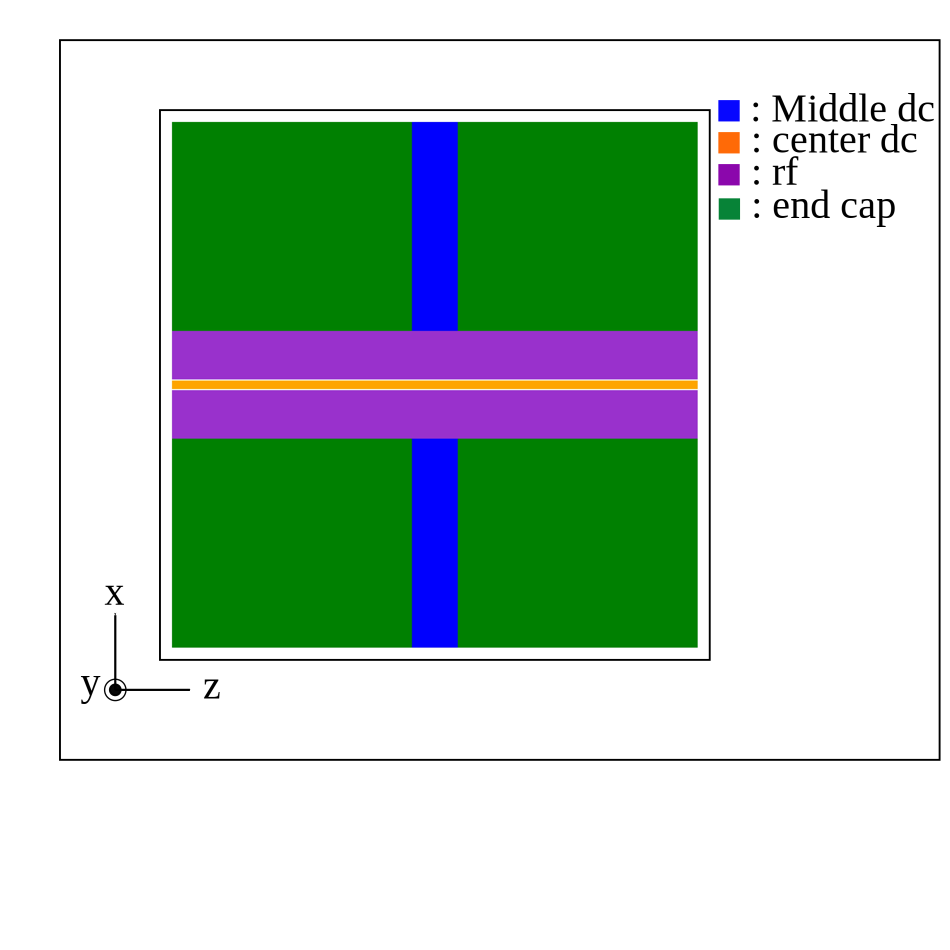
\includegraphics[width = 0.98\columnwidth]{./theory/figure/PaulTrap_3Dto2D_2DTrap.png}
			\end{center}
		\end{minipage}
	\end{center}
\end{figure}
\subsubsection{電極の仕様}
\begin{figure}[h]
	\begin{center}
		\includegraphics[width = 0.5\linewidth]{./theory/figure/named_electrode.png}
		\caption{本実験で使用するプレーナートラップの電極モデル}
		\label{fig:Named_PlannerTrap}
	\end{center}
\end{figure}
\subsubsection{矩形電極が作る静電ポテンシャル}
\begin{figure}[h]
	\begin{center}
		
\includegraphics[width = 0.5\linewidth]{./theory/figure/Potential_of_rect-electrode.png}
		\caption{$(z_1,x_1),(z_2,x_2)$で指定される矩形が任意の点$(x,y,z)$に形成する静電ポテンシャル}
		\label{fig:Potential_from_rect-electrode}
	\end{center}
\end{figure}
\begin{align}\label{eq:rectangle_electrode}
	\phi(x,y,z) = \frac{V}{2\pi} \left\lbrace \arctan \left[ \frac{(x_2 - x)(z_2 - z)}{y\sqrt{y^2 + (x_2 - x)^2 + (z_2 - z)^2}}\right] - \arctan \left[ \frac{(x_1 - x)(z_2 - z)}{y\sqrt{y^2 + (x_1 - x)^2 + (z_2 - z)^2}} \right]  \right.  \notag \\ 
	\left. -\arctan \left[ \frac{(x_2 - x)(z_1 - z)}{y\sqrt{y^2 + (x_2 - x)^2 + (z_1 - z)^2}}\right] + \arctan \left[ \frac{(x_1 - x)(z_1 - z)}{y\sqrt{y^2 + (x_1 - x)^2 + (z_1 - z)^2}} \right]  \right\rbrace 
\end{align}
\subsection{Mathematicaによるシミュレーション}
\subsubsection{DCポテンシャル}
\Eq{rectangle_electrode}より,dc電圧を計算するためには電極モデルを矩形の形に分割する必要がある.Mathematica上における電極の分割の様子を\Fig{rect_electrode}に示す.
\begin{figure}[h]
	\begin{center}
		\includegraphics[width = 0.4\linewidth]{./theory/figure/named_rect_electrode.png}
	\end{center}
	\caption{a}
	\label{fig:rect_electrode}
\end{figure}
各dc電極によってプレーナートラップ上の点$(x,y,z)$に形成される静電ポテンシャル$\Phi_{\rm DC}(x,y,z)$は,分割した各矩形が$(x,y,z)$に形成する静電ポテンシャルの重ね合わせで
\large
\begin{align}
	\Phi_{\rm DC}(x,y,z) = \phi_{\rm End1} + \phi_{\rm End2} + \phi_{\rm End3} &+ \phi_{\rm End4} + \phi_{\rm Mid1} + \phi_{\rm Mid2} \notag \\
	&+ \phi_{\rm Side1} + \phi_{\rm Side2} + \phi_{\rm center},
\end{align}
\normalsize
と表すことができる.
\begin{figure}[h]
			\begin{center}
				\includegraphics[width = 0.7\linewidth]{./theory/figure/PlannarTrap_3D_z=0.png}
			\end{center}
\end{figure}
\begin{figure}[h]
	\begin{center}
		\begin{minipage}{0.45\linewidth}
			\begin{center}
				\includegraphics[width = 1.2\columnwidth]{./theory/figure/dc_potential_example.png}
			\end{center}
		\end{minipage}
		\begin{minipage}{0.45\linewidth}
			\begin{center}
			\begin{tabular}{c|c} \hline \hline
				電極 & 印加電圧 ()V) \\ \hline
				End1 & 1.41 \\ \hline
				End2 & 1.41 \\ \hline
				End3 & 1.41 \\ \hline
				End4 & 1.41 \\ \hline
				Mid1 & -1.532 \\ \hline
				Mid2 & -1.532 \\ \hline
				Side1 & 0.222 \\ \hline
				Side2 & 0.222 \\ \hline
				center & 0.225 \\ \hline
			\end{tabular}
			\end{center}
		\end{minipage}
	\end{center}
\end{figure}
\subsubsection{Single-wellにおけるrf擬ポテンシャル}
\subsubsection{Double-wellにおけるrf擬ポテンシャル}
\subsection{レーザー冷却}
\subsection{画像処理によるイオン捕獲位置と電場の算出}
Pythonで,OpenCVとNumpyを使って画像処理を行うことでイオンの位置と,イオンの位置における電場の算出を行う.
\subsubsection{グレースケール化,二値化}
\subsubsection{イオンの検出および,捕獲位置と電場の算出方法}